\chapter{Open Source Anonymous Credentials Benchmark Library}



\subsection{Core Research Problem}
The central challenge we’re solving is: How can we establish a fair, standardized, and practical performance evaluation framework for Attribute-Based Anonymous Credential (ABC) schemes to accelerate their real-world adoption? 

There are two major gaps in the current literature:
\begin{enumerate}
    \item Efficiency Comparisons: What are the real performance differences between older and newer anonymous credential schemes when tested under identical conditions (e.g., same hardware, security parameters, and libraries)?

    \item Impact of Optimizations: How do cryptographic library optimizations—like Multi-Scalar Multiplication (MSM), batch verification, or Miller-Loop pairing optimizations—affect the practical efficiency of these schemes compared to their theoretical complexity?
    
\end{enumerate}
This problem arises because current evaluations use different programming languages (Python, C++, Rust), libraries (Arkworks, Ethereum PyEcc), and optimization choices, creating incomparable results. Consistent benchmarks are needed to compare and select a scheme fairly. 



\subsection{Core Contributions}

\begin{enumerate}
    \item Rich Experimental Data for the most popular state-of-the-art ABCs and an Open-source Anonymous Credentials Benchmark Library written in Rust for ongoing fair comparisons. 

    \item Practical Efficiency Optimization Data: Showing the impact of Schnorr proofs using MSM scaling sublinearly rather than linearly as previously thought. 

    \item Random Linear Combination Proof Aggregation (Schnorr proofs, pairings)

    \item Use-case experimental data for zero-knowledge proof statements

    Speedup techniques in rust library
    % https://github.com/sampolgar/anonymous-credentials/blob/a7cc7d199b7fe54a5863e20bac44f1aee538a58a/ps_utt_ts/src/credential.rs#L94
    
\end{enumerate}


Anonymous Credentials serve as the backbone of privacy-preserving identity systems. 

Since their inception, Anonymous Credentials have primarily been academic works; however, with the increasing need for governments and organizations to migrate secure digital identity infrastructure, for example, in the US, 13 states have interoperable mobile digital driving licenses \cite{aamva_jurisdiction_nodate} with 30 more states in consideration, in addition to the EU's eIDAS framework requiring all member states to have such infrastructure by 2026 \cite{european_parliament_meps_2024}. In light of this, there are products from Microsoft \cite{microsoft_microsoft_2025}, AWS \cite{aws_verifiable_nodate}, and \cite{dock_labs_dock_nodate} enabling this technology in addition to standardisation efforts at W3C \cite{w3c_verifiable_2025, w3c_decentralized_2022}

Therefore, the urgent question is, what is this technology's privacy/security cost? There are constant trade-offs between privacy, security, functionality, and efficiency. Improving privacy and security comes at the expense of functionality and efficiency, and vice versa. To answer this, we have built an Open-Source Anonymous Credentials Benchmark Library and (thus far) built 6 different schemes with the goal of fair comparison. We show why previous benchmark analyses are not fair and furthermore we show our analysis of using efficient practical cryptography libraries.  

Previous deployments like IBM's Idemix \cite{camenisch_design_2002} and IRMA \cite{fischer-hubner_towards_2013} based on CL-Signatures \cite{camenisch_design_2002, cimato_signature_2003}, Hyperledger Fabric \cite{androulaki_hyperledger_2018} based on BBS+ \cite{hutchison_constant-size_2006}, Microsoft's U-Prove \cite{dunkelman_formal_2016} based on Brands' signatures \cite{brands_rethinking_2000}, were deployed in pilot programs \cite{dunkelman_formal_2016}, and proved that these systems were secure, private and feature-rich, but inefficient for widespread adoption. Their implementations were based on early constructions we label as "previous generation" and lacked efficient credential verification procedures required for the expected user experience needed for large-scale uptake, which we illustrate below.

\paragraph{IRMA, Idemix and U-Prove: }

IRMA \cite{fischer-hubner_towards_2013} presents the Show+Verify for credential with 3 attributes costs about 1.3seconds (Intel Core i7-8650U CPU with 16 GB of RAM GNU/Linux) in \cite{zhang_passo_2021}

\cite{habib_evaluation_2016}: presents a more thorough evaluation of the Show+Verify algorithms:
Idemix presents Show + Verify algorithm for 1,2,3 credentials as 110ms, 220ms, 450ms
U-Prove presents Show + Verify algorithm for 1,2,3 credentials as 180ms, 460ms, 600ms
Furthermore, they show functionality use-case like selective disclosure (400ms for 1 attribute selective disclosure and 670ms for 2 attributes selective disclosure) and committed attribute equality (120ms). 

The gap we see here is that 
- doesn't take batch verification into account.
- selective disclosure costs minimal overhead. (under 1ms)
- attribute equality costing minimal overhead (under 1ms)
- Newer schemes \cite{camenisch_anonymous_2016, tomescu_utt_2022} reduce pairing operations in the signature construction itself, coupled with cryptography library improvements reduce all metrics significantly. 
This hasn't been illustrated properly. 

There is a gap in practical evaluation analysis for newer state-of-the-art constructions which we provide benchmarks for.



For Anonymous Credential and Privacy-Preserving Identity there is no library to help people learn the differences between constructions, what they can use or can't use and how they differ from a practical / functional implementation standpoint. 

Our contributions
1. built opensource library framework for SOTA anonymous credentials and benchmarked against each other in rust
2. Demonstrate that schnorr proofs which are usually "slandered" in academic papers for being linear in the size of the proven attributed are in-fact sublinear in practice due to MSM techniques
3. we show the speedup from batch / windowing schnorr proofs 
4. Show the computation reduction in pairings when using miller loop intermediate computation rather than computing and epxonentiating GT points



The Anonymous Credential field lacks standardized fair comparisons between the leading schemes (particularly BBS+ \cite{hutchison_constant-size_2006} and PS \cite{sako_short_2016}) and their newer variants \cite{camenisch_anonymous_2016}, \cite{tomescu_utt_2022}. Previous evaluations attempt to compare different schemes - although they might use consistent security parameters, variation in programming languages of the implementations (Python, C++, Rust), their underlying cryptography libraries (Arkworks, Ethereum PyEcc), and use of optimizations such as like Multi-Scalar Multiplication, Miller Loop Pairings, and Batch Techniques make fair comparison difficult to quantify. 



Our first contribution is to show the key cryptographic operations for ABC systems and present the most efficient scheme in terms of the most used operation (Show + Verify). 
Our second contribution is demonstrating the gap between theoretical and practical cryptography by implementing speedup techniques for critical operations and demonstrating our practical analysis. Our analysis is useful outside of Anonymous Credentials.
\begin{enumerate}
    \item First, we show that implementing a Schnorr protocol to prove knowledge of committed exponents scales sublinearly in the size of the attribute length (contrary to the theoretical analyses in most literature) - importantly, before making claims on performance enhancements against previous "linear" schemes, it's imperative for new schemes to compare under these assumptions rather than pure theoretic. 

    \item Second, we show a batch verification technique for multiple individual schnorr proofs improving verification time by 50\%. Demonstrate a batch verification method of individual schnorr proofs (useful in the threshold system where a user commits to each message individually, the verifier can create random linear combination and verify that $(ps_utt_ts_src_signer_batch_verify)$

    \item third, we show that pairing-based credentials significantly improve with optimized Miller-Loop implementations. Transforming a pairing equality check from this to this means a speedup of X. 
\end{enumerate}



\section{Bridging the Gap with an Open-Source Library}

Anonymous credential systems promise privacy-preserving identity solutions, yet practitioners often lack accessible tools to understand the practical differences between constructions like Schnorr-based proofs and pairing-based systems. Existing literature focuses heavily on theoretical complexity, leaving an educational gap in functional implementation details—such as what systems can or cannot do in real-world scenarios and how they perform under specific use cases. To address this, we developed an open-source library framework in Rust, implementing state-of-the-art (SOTA) anonymous credential constructions and benchmarking them against each other.

This library serves as a standardized toolkit, enabling practitioners to explore how different systems handle use cases like decentralized identity or Sybil-resistant voting. By providing empirical performance data alongside functional insights, it clarifies trade-offs that theoretical analyses often overlook. For example, while academic papers may emphasize asymptotic complexity, our benchmarks reveal how optimizations shift these boundaries in practice, making the library a valuable educational and practical resource.

Open-Source Benchmarking Framework

We developed the first standardized open-source tooling for fair comparison of anonymous credential schemes, tackling inconsistencies in previous academic evaluations. This framework empowers researchers and industry practitioners to make informed implementation decisions using quantitative performance metrics, moving beyond unfair practical claims or purely theoretical analysis. By enabling reliable and consistent assessments, it accelerates both research advancements and practical adoption of privacy-preserving technologies.










\section{New Generation Anonymous Credentials}
The performance comparison in Table \ref{tab:anon_creds_performance_old_gen_vs_new} demonstrates that newer anonymous credential schemes, such as BBS+2016 \cite{camenisch_anonymous_2016} and PS-UTT22 \cite{tomescu_utt_2022}, outperform older schemes like BBS+06 \cite{hutchison_constant-size_2006} and PS16 \cite{sako_short_2016} by shifting zero-knowledge proofs from the target group $(\mathbb{G}_T)$ to the source group ($\mathbb{G}_1)$\footnote{CL04 \cite{hutchison_signature_2004} is included in previous generation}. For 30 attributes, older schemes require computing over 3$\ell$, and 2$\ell$ $\G_T$ points respectively with Show and Verify times of 39.21 ms (BBS+06) and 32.78 ms (PS16). In comparison, newer schemes compute only in $\G_1$ and minimize pairings, achieving times of 5.72 ms and 5.38 ms—speedups of 6.85x and 6.09x, respectively. These improvements maintain full functionality, including selective disclosure and unlinkability, and rely on standard security assumptions, enhancing the practicality of anonymous credentials for digital identity systems.

\begin{table}[h]
\centering
\caption{Performance Comparison of Anonymous Credential Schemes for Show and Verify Algorithms ($\ell = 30$ Attributes)}
\label{tab:anon_creds_performance_old_gen_vs_new}
\begin{tabular}{|l|c|c|c|c|c|c|}
\hline
\textbf{Scheme} & \textbf{ZKPoK}  & \textbf{Show (ms)} & \textbf{Verify (ms)}  & \textbf{Show + Verify (ms)} & \textbf{Speedup} \\
\hline
BBS+06 & $\mathbb{G}_T$ & 12.91  & 26.30 & 39.21 & -- \\
\hline
BBS+2016 & $\mathbb{G}_1$ & 3.15  & 2.57 & 5.72 & 6.85x over BBS+ 06 \\
\hline
PS16 & $\mathbb{G}_T$ & 16.23  & 16.55 & 32.78 & -- \\
\hline
PS-UTT22 & $\mathbb{G}_1$ & 1.59  & 3.79 & 5.38 & 6.09x over PS16 \\
\hline
\end{tabular}
\end{table}


\textbf{Threshold}
Do a Table comparing Threshold Keys from TACT, Us, and BBS+




\textbf{Crypto Library Optimizations}
Do a Table showing 
Single Pairing
Miller Loop + Final Exponentiation
G1 Exponentiation, Addition
G2 Exponentiation, Addition
GT Exponentiation, Addition












































\subsection{ABC Performance Comparison}


\begin{table}[htbp]\label{abc-performance-combined-table}
\centering
\caption{Performance of Anonymous Credential Operations (time in ms), $n$ is attribute count}
\begin{tabular}{@{}p{1.2cm}*{5}{>{\centering\arraybackslash}p{1.6cm}}@{}}
\toprule
$n$ & \cite{hutchison_constant-size_2006} & \cite{camenisch_anonymous_2016} & \cite{sako_short_2016} & \cite{tomescu_utt_2022} \ref{sec:rerandsig_g1} & Our Improved \ref{rerandsig_g2} \\
\midrule
\multicolumn{6}{c}{\textbf{Obtain}}  \\
\midrule
\textbf{2} & 0.51 & 0.90 & 0.66 & 0.25 & \textbf{0.23} \\
\textbf{5} & 0.65 & 1.00 & 0.66 & 0.28 & \textbf{0.27} \\
\textbf{10} & 0.67 & 1.13 & 0.82 & 0.36 & \textbf{0.31} \\
\textbf{15} & 0.78 & 1.26 & 0.87 & 0.37 & \textbf{0.36} \\
\textbf{20} & 0.86 & 1.38 & 0.94 & \textbf{0.41} & \textbf{0.41} \\
\textbf{30} & 1.07 & 1.63 & 1.11 & 0.51 & \textbf{0.49} \\
\midrule
\multicolumn{6}{c}{\textbf{Issue}}  \\
\midrule
\textbf{2} & 1.25 & \textbf{0.72} & 1.48 & 1.27 & 2.99 \\
\textbf{5} & 1.66 & \textbf{0.75} & 1.79 & 1.66 & 3.31 \\
\textbf{10} & 2.33 & \textbf{0.83} & 2.54 & 2.35 & 4.00 \\
\textbf{15} & 2.98 & \textbf{0.84} & 3.23 & 3.03 & 4.64 \\
\textbf{20} & 3.96 & \textbf{0.90} & 3.79 & 3.66 & 5.88 \\
\textbf{30} & 4.97 & \textbf{0.94} & 5.16 & 5.10 & 6.86 \\
\midrule
\multicolumn{6}{c}{\textbf{Show}}  \\
\midrule
\textbf{2} & 5.39 & 2.31 & 3.20 & \textbf{1.14} & 1.29 \\
\textbf{5} & 6.05 & 2.42 & 3.15 & \textbf{1.16} & 1.29 \\
\textbf{10} & 7.44 & 1.71 & 4.53 & \textbf{1.22} & 1.33 \\
\textbf{15} & 8.86 & 2.71 & 6.14 & 1.40 & \textbf{1.37} \\
\textbf{20} & 11.88 & 1.88 & 7.66 & \textbf{1.41} & 1.51 \\
\textbf{30} & 12.91 & 3.15 & 16.23 & \textbf{1.37} & 1.59 \\
\midrule
\multicolumn{6}{c}{\textbf{Verify}}  \\
\midrule
\textbf{2} & 7.59 & 2.18 & 4.57 & 2.47 & \textbf{1.79} \\
\textbf{5} & 9.25 & 2.25 & 5.52 & 2.73 & \textbf{2.01} \\
\textbf{10} & 11.09 & \textbf{2.25} & 7.10 & 3.16 & 2.44 \\
\textbf{15} & 13.96 & \textbf{2.30} & 8.62 & 3.47 & 2.72 \\
\textbf{20} & 16.93 & \textbf{2.34} & 9.88 & 3.84 & 3.21 \\
\textbf{30} & 26.30 & \textbf{2.57} & 16.55 & 4.67 & 3.79 \\
\midrule
\multicolumn{6}{c}{\textbf{Issuing Phase Total (Obtain + Issue)}}  \\
\midrule
\textbf{2} & 1.76 & 1.62 & 2.14 & \textbf{1.53} & 3.22 \\
\textbf{5} & 2.31 & \textbf{1.76} & 2.45 & 1.95 & 3.57 \\
\textbf{10} & 3.00 & \textbf{1.96} & 3.37 & 2.71 & 4.31 \\
\textbf{15} & 3.75 & \textbf{2.10} & 4.10 & 3.40 & 5.00 \\
\textbf{20} & 4.82 & \textbf{2.29} & 4.74 & 4.06 & 6.28 \\
\textbf{30} & 6.04 & \textbf{2.57} & 6.27 & 5.60 & 7.35 \\
\midrule
\multicolumn{6}{c}{\textbf{Showing Phase Total (Show + Verify)}}  \\
\midrule
\textbf{2} & 12.98 & 4.48 & 7.77 & 3.61 & \textbf{3.08} \\
\textbf{5} & 15.30 & 4.67 & 8.68 & 3.90 & \textbf{3.30} \\
\textbf{10} & 18.53 & 3.96 & 11.62 & 4.38 & \textbf{3.77} \\
\textbf{15} & 22.82 & 4.22 & 14.76 & 4.87 & \textbf{4.09} \\
\textbf{20} & 28.81 & 5.01 & 17.53 & 5.25 & \textbf{4.72} \\
\textbf{30} & 39.21 & 5.72 & 32.77 & 6.04 & \textbf{5.37} \\
\bottomrule
\end{tabular}
\end{table}































\section{Practical Proof Analysis}
\subsection{Sigma Protocols}\label{sigma-protocol-analysis}
Many schemes refer to sigma protocol as having linear size proofs. 
While this is true in theory, using multi-scalar-multiplication, a popular algorithm in many cryptographic libraries, we show that sigma protocols are, in fact, sublinear rather than linear when message size doubles.

These findings support the hypothesis that practical efficiency is substantially better than theoretical complexity would suggest when using MSM in Schnorr protocols and thus the proof protocols in PS and BBS+ based anonymous credentials are sublinear in practice.

\begin{figure}
    \centering
    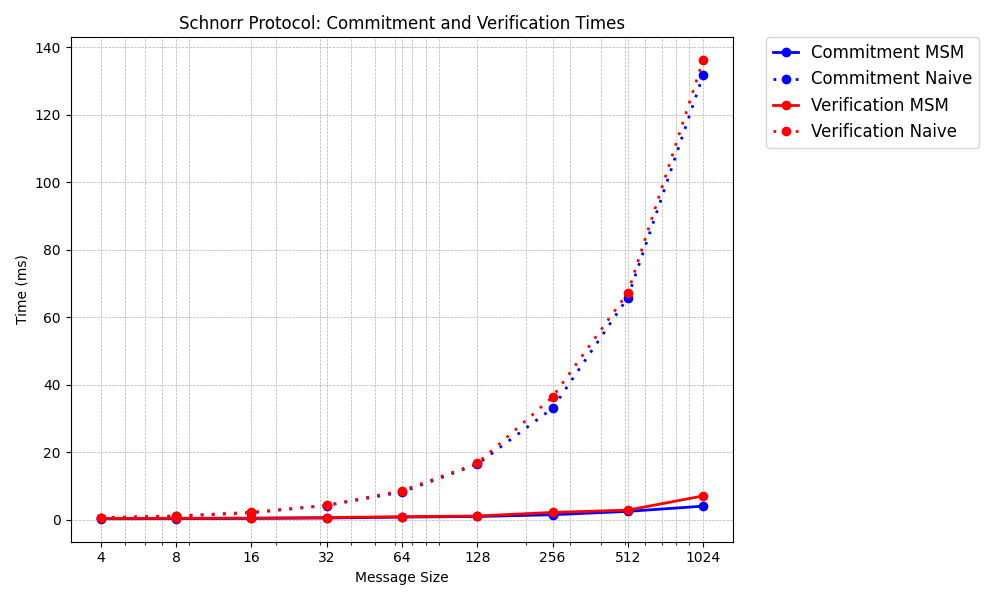
\includegraphics[width=0.75\linewidth]{schnorr_msm_no_msm.png}
    \caption{Schnorr Protocol - Practical Benchmarks with Multi-Scalar Multiplication}
    \label{fig:schnorr-benchmarks}
\end{figure}




\subsection{Pairing Protocols}

\begin{figure}
    \centering
    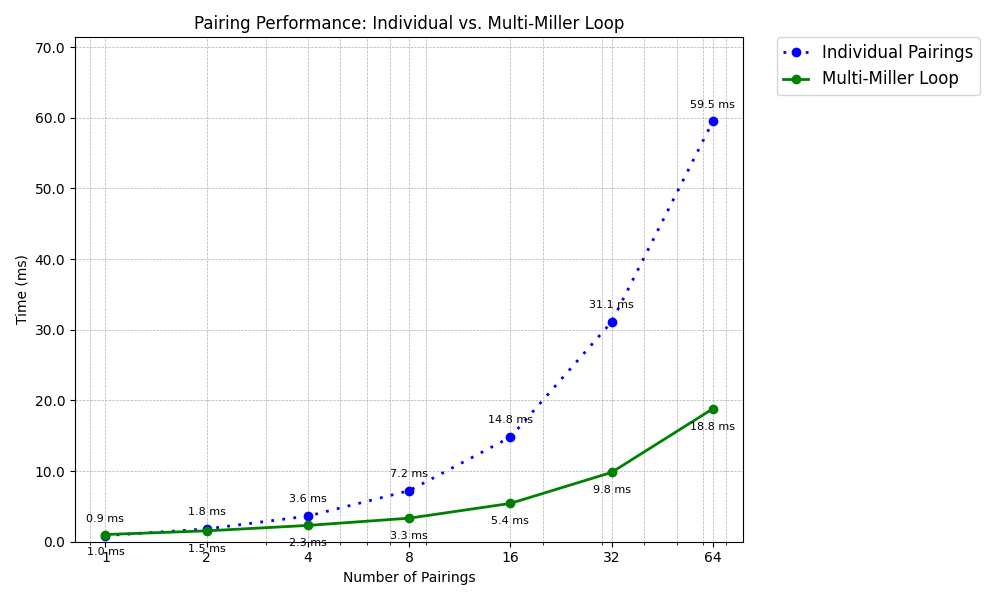
\includegraphics[width=0.75\linewidth]{pairing_comparison.png}
        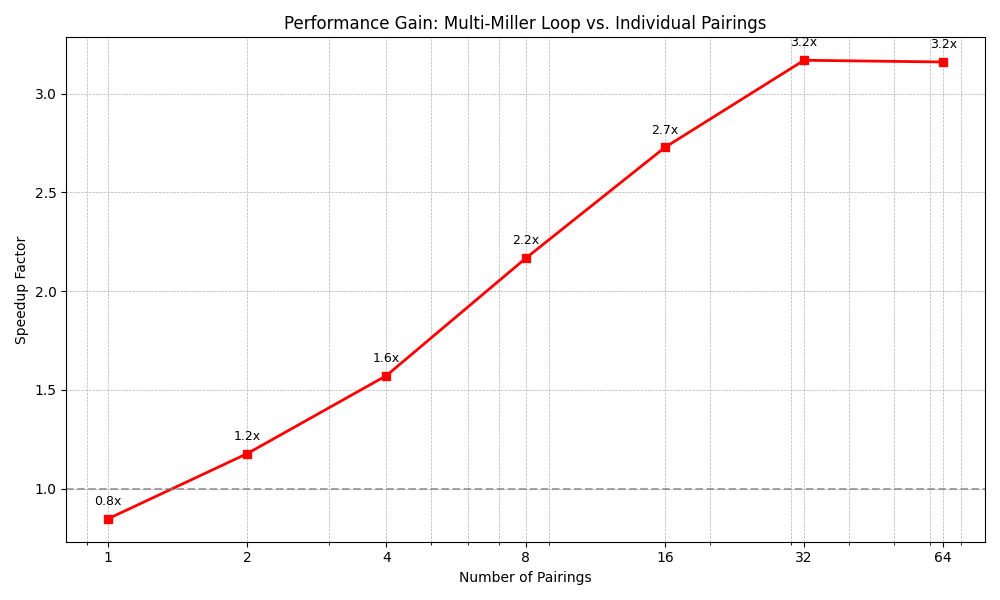
\includegraphics[width=0.75\linewidth]{pairing_comparison2.png}
    \caption{Elliptic Curve Pairings - Practical Benchmarks with Miller-Loop Intermediate Computation}
    \label{fig:enter-label}
\end{figure}




\subsection{Use-Case Case Study}

To demonstrate the practical impact of our optimizations, we compared our approach against alternative systems for the common use case of verifying credential expiration. Table~\ref{tab:expiry-comparison} presents the results for generating and verifying a proof that a credential has not expired.



\begin{table}[htbp]
\centering
\caption{Performance Comparison for Credential Operations}
\label{tab:expiry-comparison}
\begin{tabular}{lrrrr}
\toprule
\textbf{Approach} & \textbf{Scheme} & \textbf{Show (ms)} & \textbf{Verify (ms)} & \textbf{Proof Size} \\
\midrule
Simple Possession & \cite{rosenberg_zk-creds_2022} & 2 & 2 & 424B \\
& Us & 2 & 2 & \\
\midrule
Expiry & \cite{rosenberg_zk-creds_2022} & 2 & 2 & 424B \\
& Us & 2 & 2 & \\
\midrule
Linkable Show & \cite{rosenberg_zk-creds_2022} & 41 &  &  \\
& Us & 2 & 2 & \\
\midrule
Rate Limiting & \cite{rosenberg_zk-creds_2022} & 58 &  &  \\
& Us & 2 & 2 & \\
\bottomrule
\end{tabular}
\end{table}

Our evaluation reveals that our system can verify a credential's expiry status in just 3.3ms (combined Show+Verify), compared to 45-55ms for ZK-Creds approaches—a performance improvement of over 13×. This dramatic difference highlights how our optimized signature scheme and sigma protocol enables efficient predicate verification without sacrificing privacy.

Importantly, while general-purpose zero-knowledge systems provide flexibility, they introduce substantial computational overhead that makes interactive verification scenarios impractical. Our approach achieves similar expressiveness with dramatically better performance for the most common credential verification operations.


